% Save this as workflow.tex and compile with pdflatex (pdflatex workflow.tex)
```latex
\documentclass[10pt,a4paper]{article}
\usepackage[margin=1in]{geometry}
\usepackage{tikz}
\usetikzlibrary{shapes.geometric, arrows.meta, positioning, fit}

\pagestyle{empty}

% Styles
\tikzset{
  block/.style = {rectangle, draw=black, thick, rounded corners, text width=10.5cm, align=left, minimum height=11mm, inner sep=6pt},
  smallblock/.style = {rectangle, draw=black, thick, rounded corners, text width=6.5cm, align=left, minimum height=9mm, inner sep=4pt},
  decision/.style = {diamond, draw=black, thick, aspect=2, inner sep=3pt, text width=4.5cm, align=center},
  io/.style = {rectangle, draw=black, thick, rounded corners, text width=4.5cm, align=center, minimum height=8mm},
  startstop/.style = {ellipse, draw=black, thick, minimum width=4cm, minimum height=8mm, align=center},
  connector/.style = {very thick, -{Stealth[length=4mm,width=2.0mm]}},
  note/.style = {rectangle, draw=black, dashed, rounded corners, fill=gray!5, text width=3.6cm, align=center, inner sep=5pt}
}

\begin{document}

\begin{figure}[htp]
\centering
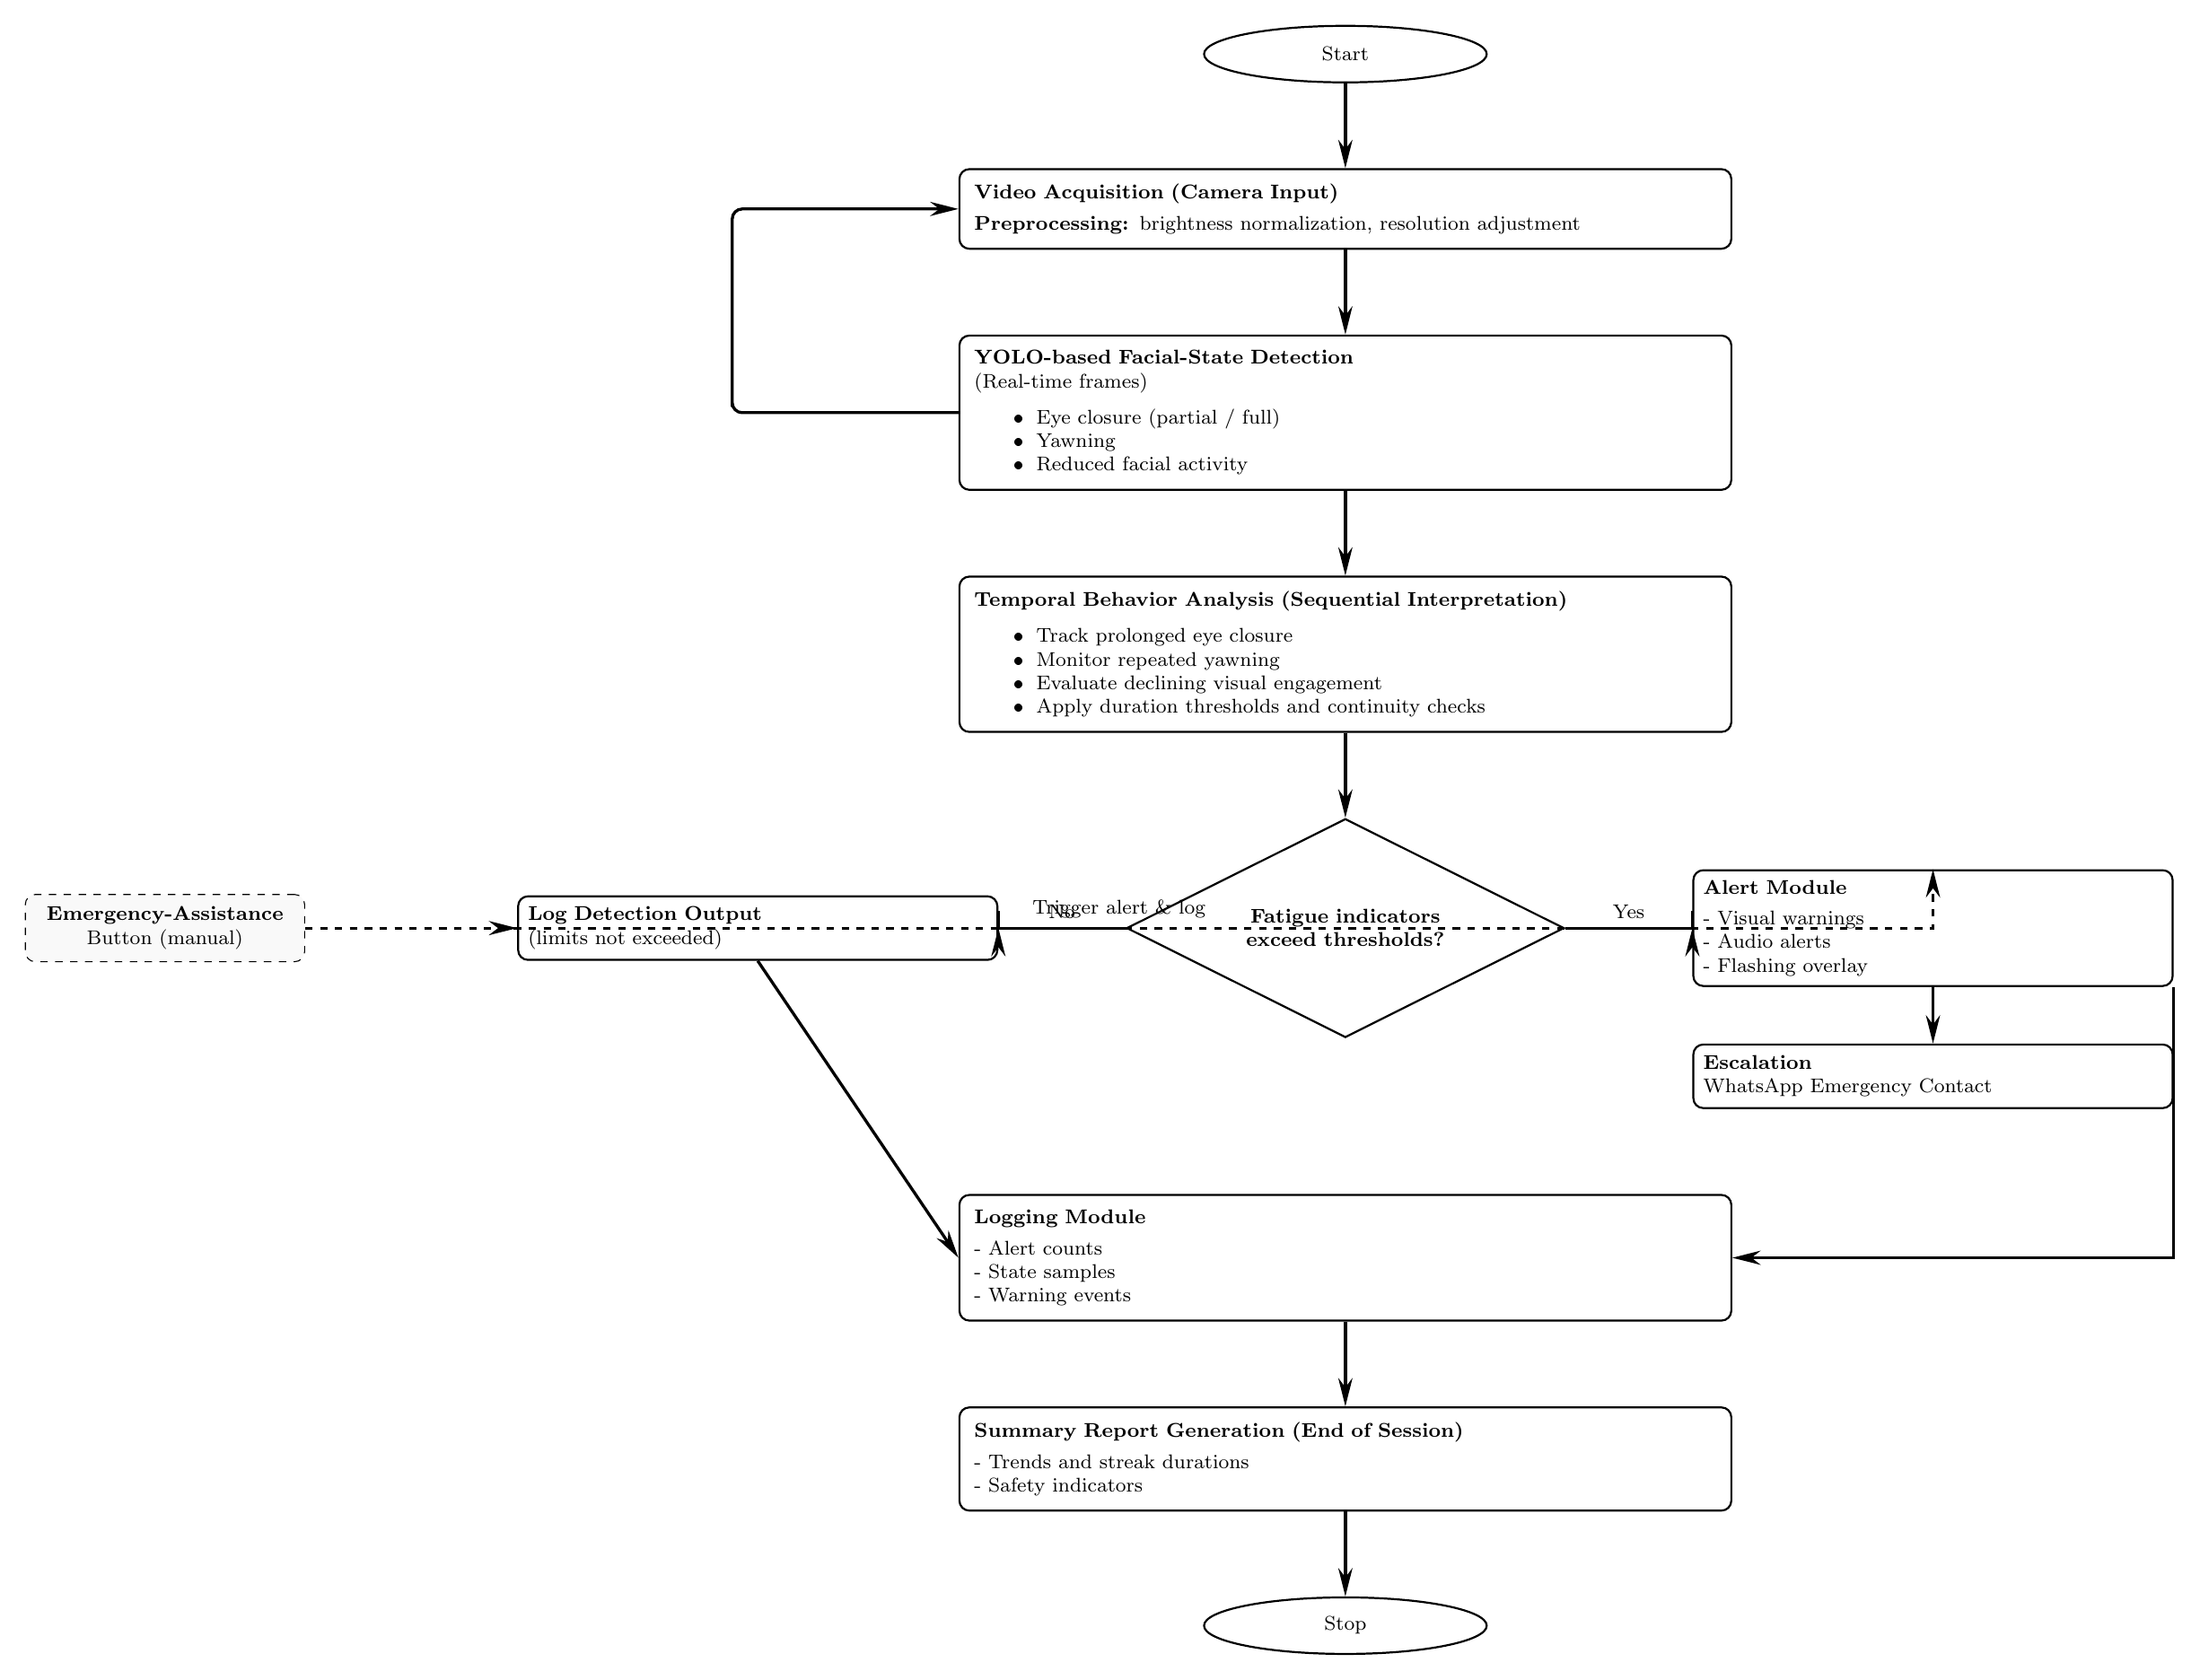
\begin{tikzpicture}[node distance=10mm and 0mm, every node/.style={font=\footnotesize}]

  % Top start
  \node (start) [startstop] {Start};

  % Video acquisition + preprocessing block
  \node (video) [block, below=12mm of start] {
    \textbf{Video Acquisition (Camera Input)}\\[3pt]
    \textbf{Preprocessing:} brightness normalization, resolution adjustment
  };

  % YOLO block
  \node (yolo) [block, below=12mm of video] {
    \textbf{YOLO-based Facial-State Detection}\\(Real-time frames)\\[3pt]
    \begin{itemize}\setlength\itemsep{0pt}\setlength\parskip{0pt}
      \item Eye closure (partial / full)
      \item Yawning
      \item Reduced facial activity
    \end{itemize}
  };

  % Temporal behaviour block
  \node (temporal) [block, below=12mm of yolo] {
    \textbf{Temporal Behavior Analysis (Sequential Interpretation)}\\[3pt]
    \begin{itemize}\setlength\itemsep{0pt}\setlength\parskip{0pt}
      \item Track prolonged eye closure
      \item Monitor repeated yawning
      \item Evaluate declining visual engagement
      \item Apply duration thresholds and continuity checks
    \end{itemize}
  };

  % Decision diamond
  \node (decision) [decision, below=12mm of temporal] {\textbf{Fatigue indicators exceed thresholds?}};

  % Alert module (right)
  \node (alert) [smallblock, right=18mm of decision] {
    \textbf{Alert Module}\\[3pt]
    - Visual warnings\\
    - Audio alerts\\
    - Flashing overlay
  };

  % WhatsApp escalation (right of alert)
  \node (whatsapp) [smallblock, below=8mm of alert] {
    \textbf{Escalation}\\
    WhatsApp Emergency Contact
  };

  % Log detection output (left)
  \node (logdet) [smallblock, left=18mm of decision] {
    \textbf{Log Detection Output}\\(limits not exceeded)
  };

  % Logging module (below decision)
  \node (logging) [block, below=22mm of decision] {
    \textbf{Logging Module}\\[3pt]
    - Alert counts\\
    - State samples\\
    - Warning events
  };

  % Summary report (below logging)
  \node (report) [block, below=12mm of logging] {
    \textbf{Summary Report Generation (End of Session)}\\[3pt]
    - Trends and streak durations\\
    - Safety indicators
  };

  % Stop node
  \node (stop) [startstop, below=12mm of report] {Stop};

  % Emergency button (left side)
  \node (emg) [note, left=30mm of logdet] {\textbf{Emergency-Assistance}\\Button (manual)};

  % Draw connections
  \draw[connector] (start) -- (video);
  \draw[connector] (video) -- (yolo);
  \draw[connector] (yolo) -- (temporal);
  \draw[connector] (temporal) -- (decision);

  % Decision yes -> alert
  \draw[connector] (decision.east) -| node[near start, above] {Yes} (alert.west);
  \draw[connector] (alert.south) -- (whatsapp.north);
  \draw[connector] (alert.south east) |- (logging.east);

  % Decision no -> logdet -> logging
  \draw[connector] (decision.west) -| node[near start, above] {No} (logdet.east);
  \draw[connector] (logdet.south) -- (logging.west);

  % Logging -> report -> stop
  \draw[connector] (logging) -- (report);
  \draw[connector] (report) -- (stop);

  % Emergency button triggers alert and logs
  \draw[connector, dashed] (emg.east) -| node[near start, above] {Trigger alert \& log} (alert.north);
  \draw[connector, dashed] (emg.east) |- node[very near start, below] {} (logdet.west);

  % Feedback arrow: YOLO detection may feed back to video (optional)
  \draw[connector, rounded corners] (yolo.west) -| ++(-3.2,0.0) |- (video.west);

  % Small labels (optional)
  \node[font=\small, below=2mm of decision] {}; % spacing

\end{tikzpicture}
\caption{Workflow of the system — overall operational flow from video acquisition through detection, temporal analysis, alerting, logging and report generation.}
\label{fig:workflow}
\end{figure}

\end{document}

```
